\documentclass[12pt,a4paper,bibliography=totocnumbered,listof=totocnumbered]{scrartcl}
\usepackage[utf8]{inputenc}
\usepackage{amsmath}
\usepackage{amsfonts}
\usepackage{amssymb}
\usepackage{graphicx}
\usepackage{fancyhdr}
\usepackage{tabularx}
\usepackage{geometry}
\usepackage{setspace}
\usepackage[right]{eurosym}
\usepackage[printonlyused]{acronym}
\usepackage{subfig}
\usepackage{floatflt}
\usepackage[usenames,dvipsnames]{color}
\usepackage{colortbl}
\usepackage{paralist}
\usepackage{array}
\usepackage{titlesec}
\usepackage{parskip}
\usepackage[right]{eurosym}
\usepackage{colortbl}
\usepackage[subfigure,titles]{tocloft}
\usepackage{subfig}
\usepackage[pdfpagelabels=true]{hyperref}
\usepackage[round]{natbib}
\usepackage{listings}
\usepackage{xcolor}


\lstset{basicstyle=\footnotesize, captionpos=b, breaklines=true, showstringspaces=false, tabsize=2, frame=lines, numbers=left, numberstyle=\tiny, xleftmargin=2em, framexleftmargin=2em, language=python}
\makeatletter
\def\l@lstlisting#1#2{\@dottedtocline{1}{0em}{1em}{\hspace{1,5em} Lst. #1}{#2}}
\makeatother

\geometry{a4paper, top=27mm, left=30mm, right=20mm, bottom=35mm, headsep=10mm, footskip=12mm}

\hypersetup{unicode=false, pdftoolbar=true, pdfmenubar=true, pdffitwindow=false, pdfstartview={FitH},
	pdftitle={Bachelorarbeit},
	pdfauthor={Alina Asisof},
	pdfsubject={Bachelorarbeit},
	pdfcreator={\LaTeX\ with package \flqq hyperref\frqq},
	pdfproducer={pdfTeX \the\pdftexversion.\pdftexrevision},
	pdfkeywords={Bachelorarbeit},
	pdfnewwindow=true,}

\pdfinfo{/CreationDate (D:20110620133321)}


\begin{document}

\titlespacing{\section}{0pt}{12pt plus 4pt minus 2pt}{-6pt plus 2pt minus 2pt}

% Kopf- und Fusszeile
\renewcommand{\sectionmark}[1]{\markright{#1}}
\renewcommand{\leftmark}{\rightmark}
\pagestyle{fancy}
\lhead{ }
\chead{ }
\rhead{\thesection\space\contentsname}
\lfoot{Software Engineering}
\cfoot{ }
\rfoot{\ \linebreak Page \thepage}
\renewcommand{\headrulewidth}{0.4pt}
\renewcommand{\footrulewidth}{0.4pt}

% Vorspann
\renewcommand{\thesection}{\Roman{section}}
\renewcommand{\theHsection}{\Roman{section}}
\pagenumbering{Roman}

% ----------------------------------------------------------------------------------------------------------
% Titelseite
% ----------------------------------------------------------------------------------------------------------
\thispagestyle{empty}
\begin{center}
	
	\vspace*{2cm}
	\Huge
	\textbf{Software Engineering}\\
\vfill
	\Large
	\textbf{Which effect does the exchange rate of the Swiss Franc and the Euro have on Swiss tourism?}\\
\vfill
	\Large
	{Prof. Dr. Philipp Zahn}\\
	\Large
	University of St. Gallen
	
\vfill


\end{center}

\begin{flushleft}	
	\vfill
	\normalsize
\textbf{Submitted by:} \\
Alina Asisof, Master of Business Innovation HSG\\
Student Number: 12-749-677\\ 
Carla Walker, Master of Business Innovation HSG\\ 
Student Number: 12-611-091\\ 

Jo\~ao Matias, Bachelor of Economics Nova SBE\\ 
Student Number: 16-601-809\\ 
\vfill
Group Project Documentation\\ 
 
\vfill
\textbf{18. January 2017}

\end{flushleft}	



\pagebreak
%list of figures 
\listoffigures
\pagebreak

% ----------------------------------------------------------------------------------------------------------
% Verzeichnisse
% ----------------------------------------------------------------------------------------------------------
% TODO Typ vor Nummer

\renewcommand{\cftfigpresnum}{Abb. }
\settowidth{\cfttabnumwidth}{Abb. 10\quad}
\settowidth{\cftfignumwidth}{Abb. 10\quad}

\titlespacing{\section}{0pt}{12pt plus 4pt minus 2pt}{2pt plus 2pt minus 2pt}
\singlespacing
\rhead{CONTENT}
\renewcommand{\contentsname}{II Content}

\phantomsection
\addcontentsline{toc}{section}{\texorpdfstring{\hspace{0.35em}Content}{Content}}
\addtocounter{section}{1}
\tableofcontents
\pagebreak

%\pagebreak


\pagebreak


% ----------------------------------------------------------------------------------------------------------
% Inhalt
% ----------------------------------------------------------------------------------------------------------
% Abstände Überschrift
\titlespacing{\section}{0pt}{12pt plus 4pt minus 2pt}{-6pt plus 2pt minus 2pt}
\titlespacing{\subsection}{0pt}{12pt plus 4pt minus 2pt}{-6pt plus 2pt minus 2pt}
\titlespacing{\subsubsection}{0pt}{12pt plus 4pt minus 2pt}{-6pt plus 2pt minus 2pt}

% Kopfzeile
\renewcommand{\sectionmark}[1]{\markright{#1}}
\renewcommand{\subsectionmark}[1]{ }
\renewcommand{\subsubsectionmark}[1]{ }
\lhead{Chapter \thesection}
\rhead{\rightmark}

\onehalfspacing
\renewcommand{\thesection}{\arabic{section}}
\renewcommand{\theHsection}{\arabic{section}}
\setcounter{section}{0}
\pagenumbering{arabic}
\setcounter{page}{1}

%--------------------
%Einleitung
%--------------------

\section{Introduction}

%What problem does our project solve ? 
%For what will our code be used? 
%Research question: What effect had the abandonment of the Swiss Franc - Euro parity of January 2015 on tourism within and outside of Switzerland? 
%How does the strong CHF influence travel behavior? 
%CHF goes up - people travel more outside of Switzerland? 
%How will we analyze this? 
%What are the tools that we are going to use? Python and Latex. 


On January 15th the Swiss National Bank decided to abandon the Swiss Franc - Euro parity of 1.20:1. The financial markets reacted immediately: The exchange rate fell drastically and one Euro temporarily was worth less than 0.8 Swiss Francs. The decision surprised experts and executives alike and evoked great concerns regarding the future competitiveness of the Swiss industries. Some of the analysis are yet to be made and conclusions to be drawn. The risen value of the Swiss currency also left the national tourism industry sorrowful, as hotel owners and owners of popular touristic attractions alike feared a diminishing number of foreign tourists and hence missing out on revenue. Our project will focus on the tourism industry: We will conduct a simple regression to see whether the Swiss exchange rate has an effect on the national tourism industry. We look at question like how tourism in the country reacts to changes in the exchange rate and how a strong Swiss Franc influences the travel behavior within and outside of Switzerland. At the end we will conclude, if we can observe an impact of the exchange rate on tourism on the basis of tourist numbers and expenses. 

We will analyze this by using a data set provided by the Federal Statistical Office. The Federal Statistical Office publishes a variety of data on tourism throughout the year. For 1998 - 2015 there is a comprehensive set of data available, gathered in form of Excel-files and officially published. A regression on the exchange rate of the Swiss Franc to Euro will be made for the years 2008 to 2015. We will therefore use financial data published at "statista.com", so both our sources are trustworthy and well known. We will compute a regression with the help of a code written in Python on Spyder. To do that, we will remotely collaborate with the help of GitHub, a platform used to write code in groups. GitHub will also help us with the coordination and collaboration challenge connected to our project.\\
For the documentation of our project we have used LateX, as it is a tool easily embedding both Python Code and different types of content. \\
\\
We will first introduce our data set and parameters. In the following chapter we will conduct the regression and present the results of our Python code. We will add a short explanation on the code, so that the code can be easily understood and reproduced. In the last part we will conclude on the tourism effects of the exchange rate and assess, to what extend the concerns expressed by hotel owners and experts were justified. 


\newpage


% ----------------------------------------------------------------------------------------------------------
% 
% ----------------------------------------------------------------------------------------------------------
\section{Datasets}



Our term paper researches the question how exchange rates, in particular the EUR-CHF exchange rate influences Swiss tourism. To analyze the question, we compared two datasets. The first one is the historical exchange rate between the Euro and the Swiss Franc. The second dataset is from the Federal Statistical Office on the chronological development of travels with overnight stays of the Swiss population from 15 years old (Swiss Federal Statistical Office, 2016). \\     


As the Swiss Exchange Rate to the Euro was falling for several years, the Swiss National Bank (SNB) of Switzerland decided on September 6, 2011 to fix the minimum exchange rate of 1.20 Franc to one Euro. The SNB declared, that the minimum exchange rate will be enforced with all the consequences and that it is willing to buy unlimited foreign exchanges (Swiss National Bank, 2011). With this action step, the Swiss National Bank reacted to the constant threat of the Swiss Economy and the risk of a deflationary trend which resulted from the massive overvaluation of the Swiss Franc. On January 15, the Swiss National Bank discontinued the minimum exchange rate of 1.20 Franc to the Euro (SNB, 2015). The Swiss National Bank declared that maintaining the minimum exchange rate for the Swiss franc against the Euro is no longer justified. The Swiss Economy which is oriented towards export and tourism, reacted with great concerns. 

\begin{figure}[htbp] 
  \centering
     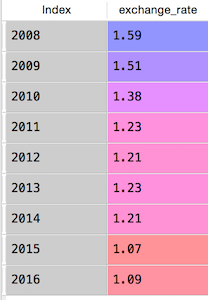
\includegraphics[width=0.3\textwidth]{exchange_variable}
  \caption{\textit{Variable explorer in Python}}
  \label{fig: figure1}
\end{figure}

For our term paper, we took data from Statista, a statistics portal. The statistic chosen displays the annual exchange rate (standardized measure) of the Euro to the Swiss franc (EUR-CHF), according to the data of the European Central Bank. We only considered the data from the years 2008 to 2015. In 2008, for example, the Euro to Swiss franc exchange rate was equal to approximately 1.59, which means that one euro could buy 1.59 Swiss francs. In 2015, the Euro to Swiss franc exchange rate was equal to approximately 1.07, which means that one euro could only buy 1.07 Swiss francs (Statista, 2016). This resulted in huge value losses of European valuta and made the Swiss Franc savings more valuable.

The Federal Statistical Office provides a detailed dataset of the chronological development of travels with overnight stays. This dataset contains statistical information regarding the private domestic tourism expenses and private tourism expenses of the Swiss Nationals abroad per person and day. This information includes accommodation expenses as well as money spent on meals and drinks, transportation costs and other costs. The dataset also includes information on the amount of foreign travels (travels outside of Switzerland) and travels within the boundaries of the Swiss territory in thousand. We can therefore compare, whether either of the parameters changes with regard to the other when plotted against the exchange rate. The dataset is available as an Excel-table for download. The table also contains information such as the number of travels per person, the demographics of the people who travelled and more detailed information about the travels itself, including the duration, the purpose, the type of accommodation, the means of transport, the destination and more. \\     

For our research, we decided on the following parameters: expenses - domestic and abroad, number of travels - in Switzerland and abroad. The goal is that further parameters can be analyzed in relationship with the exchange rate through our code very easily. 

%Here comes something on Data Management. Maybe a short explanation of what we did with the excel files? 


\newpage
\section{Constructing a Linear Regression}
A Linear regression assumes a linear relation between the input variables (X) and the single output variable (Y). We assume a linear change in the expenses people are willing to make abroad and "at home" with respect to the value of the currency. We also expect a linear relation between the exchange rate as a relative value of one currency to the other and the number of travels. A low exchange rate, e.g. 1.07 CHF/Euro means, that traveling abroad becomes comparably cheaper and traveling domestically becomes relatively more expensive. We hence expect a positive linear relation between exchange rates and domestic travels and a negative linear relation between exchange rates and travels abroad. We expect similar relations between the exchange rate and domestic expenses resp. expenses abroad: A rising exchange rate hinders people of spending money abroad whereas a sinking exchange rate should theoretically foster the spending of money abroad.\\ We tested this theoretical approach by executing a linear regression via Python. \\
\subsection{Data Management}
In order to execute a regression written in Python, we first set up a file to manage the data. We parsed multiple Excel files to combine the data. The output is a table with a column for the data in each excel file, with each row corresponding to a given year. Concretely, the parameters described above appear in a single merged file in columns indexed by year. 

We wanted to automate as much as possible in our python code. This translated into the following objective: the researcher only needs to save the Excel files with a specific simple setup and then the code arranges all those files and makes the data usable for the calculations required. The basic setup of the file is characterized by a row listing the years and each one of the other rows listing the research variables. To our knowledge this is the process that automates the most of the data management, given variables presented in the same way.
\\      
\subsection{Reading the Data}

To read our data into our python code, we first had to import some software libraries such as \textit{pandas} which is providing us with easy to use data structures and data analysis. We also imported the \textit{glob} module, since we use a wildcard pattern to import our data. 

In the end we set the directory of the data import files and used the module \textit{glob} to create a list with all the research variables files in the data folder:
\ \\
\begin{verbatim}
import pandas as pd
import glob
\end{verbatim}
\textcolor{gray}{\textit{\# set directory of data import files}}\\ 
\textcolor{gray}{\textit{\# @var curr = files directory}}
\begin{verbatim}
curr = "../softwareengineering/Data/RV*.xlsx"
glob.glob(curr)
\end{verbatim}
\ \\
It is important to adjust the directory of the data import files. Otherwise, the code will not run. As a next step we created a data frame. This is necessary to append all the different rows with our data according to the same year in columns. The reason why we split the code into different parts and created data frames is not only for better comprehension but also to make sure, that the code still works in case the Excel file's face changes. Hence, we can add more data and rows in the excel file without the code returning errors. The data frame was created as follows:
\ \\
\begin{verbatim}
dataset = pd.DataFrame()
for f in glob.glob(curr):
df =p d.read_excel(f)
dataset = dataset.append(df, ignore_index=True)
dataset = dataset.set_index("year").T
\end{verbatim}
\textcolor{gray}{\textit{\# bug fixing}}
\begin{verbatim}
dataset = dataset.reset_index().rename(columns={"index" : "year"})
dataset.columns.name = None
dataset.set_index("year", inplace = True)
\end{verbatim}
\ \\
With this piece of code, we can now print the transposed data set and receive a table in our console in Spyder :

\begin{figure}[htbp] 
  \centering
     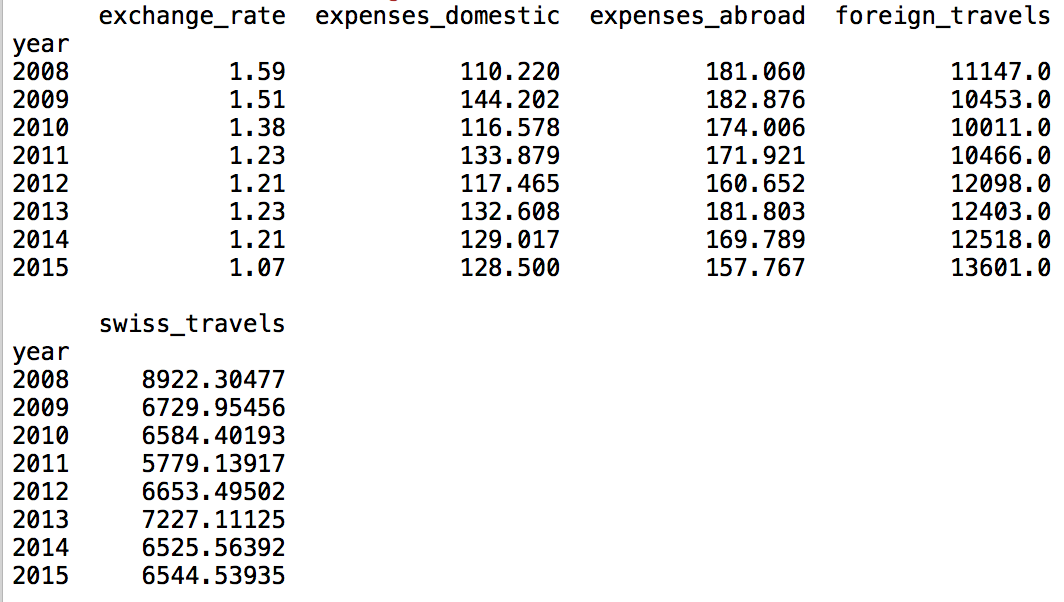
\includegraphics[width=0.5\textwidth]{data_table}
  \caption{\textit{Data set according to parameters and year}}
  \label{fig: figure2}
\end{figure}

\newpage
\subsection{Plotting}
With \textit{sklearn} which is a machine learning library allowing for regression and mean computations and interoperating with another scientific library called \textit{NumPy} we can now execute high-level mathematical functions like coefficients. With \textit{matplotlib} which is a plotting library, we can plot the results after importing the dataset. 
\ \\
\begin{verbatim}
from sklearn import linear_model
import matplotlib.pylot as plt
import numpy as np
\end{verbatim}
\textcolor{gray}{\textit{\# import dataset from the data management module}}
\begin{verbatim}
from datamanagement import dataset
\end{verbatim}
\ \\
Now we are ready to plot the variables against each other. We defined, that \verb|(x_df)| is the data frame column for the exchange rate, whereas the \verb|(y_df)| is the data frame column for the y-value, which can be exchanged for any of the four parameters chosen. 
\ \\
\begin{verbatim}
x_df = dataset.loc[:,["exchange_rate"]]
y_df = dataset.loc[:,["swiss_travels"]]
\end{verbatim}
\ \\

Now we can run the regression, plot the results and ask our interface to return the graphs:
\ \\
\begin{verbatim}
regr = linear_model.LinearRegression()
regr.fit(x_df, y_df)
\end{verbatim}
\textcolor{gray}{\textit{\# plot outputs and show the graph}}
\begin{verbatim}
plt.scatter(x_df, y_df, color='black')
plt.plot(x_df, regr.predict(x_df), color='blue', linewidth=3)
plt.show()
\end{verbatim}
\ \\
The plotted graph for the Swiss travels in dependence of the exchange rate is displayed as follows: 
\begin{figure}[htbp] 
  \centering
     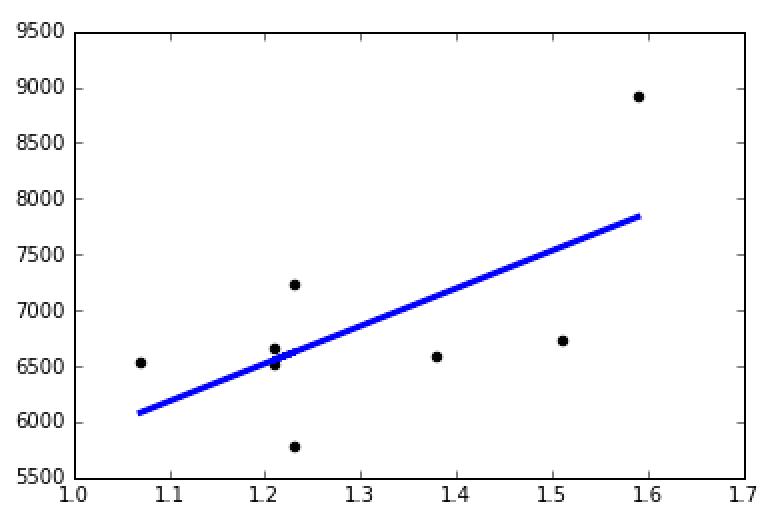
\includegraphics[width=0.6\textwidth]{lr_swiss_travels.png}
  \caption{\textit{Regression of number of Swiss travels}}
  \label{fig: figure3}
\end{figure}

We can now see the relation between the variables for every single column just by changing the \textit{y}-Variable. We can hence recreate the regression with any of the four parameters we have already described in the dataset chapter. 
\newpage
\subsection{Coefficients}
In a last step, we conduct the coefficients, the mean square error and the variance:
\ \\
\begin{verbatim}
print('Coefficients: \n', regr.coef_)
print("Mean squared error: \%.2f" \% np.mean((regr.predict(x_df) - y_df)
 ** 2))
print('Variance score: \%.2f' \% regr.score(x_df, y_df))
\end{verbatim}
\ \\
For the number of Swiss travels we obtained a coefficient of 3372, meaning that, on average, for an increase of 0.1 units in the exchange rate, the number of travels within Switzerland increases for 337 thousand (values of number of travels in thousands). The explained variance score is 0.41, which is a fairly good indicator of the predictability of this simple linear regression. Almost half of the variance is explained, and half is not. The mean error (square root of the mean squared error) is 659, on average, for a unit change in the variation of the exchange rate, the deviation from reality would be 659 thousand travels. In a coefficient of 3372 thousands, it enables a reasonable confidence interval. \\

For travels to foreign countries, -4983 is the coefficient. Meaning that, on average, for an increase in 0.1 units in the exchange rate leads to a decrease of 498 thousand travels to foreign countries (values of number of travels in thousands). The variance score is similar to the one for Swiss travels, 0.48, and the error is higher. The predictability seems higher, but the error is also higher. \\

Analyzing the relationship between the daily expenses per person abroad in private travels and the exchange rate, we observe a positive coefficient of 41.57, meaning that, for each decimal increase in the exchange rate, these daily expenses increase, on average, 4.2 francs. The mean squared error, 33.26, is considered small. Considering also an explained variance of 0.58, it is the most predictable variable we have, so the most reliable. \\

The domestic expenses, also given in a daily measure per person considering only private travels is less reliable to derive conclusions from. The variance score is 0.04, the regression will have a difficult time to explain future values. This can be due to abnormal values resulting from other factors not considered in the simple linear regression. \\

In the explanation of the coefficient a decimal interpretation was made, because it is more likely to have those kind of variations and therefore the interpretation is easier to understand.   

\section{Analysis}
For the analysis of the question on how the exchange rate between the Swiss Franc and the Euro influences the Swiss tourism we will have a look at the regression. 

\begin{figure} [htbp]
\centering
    \subfloat[Foreign travels]{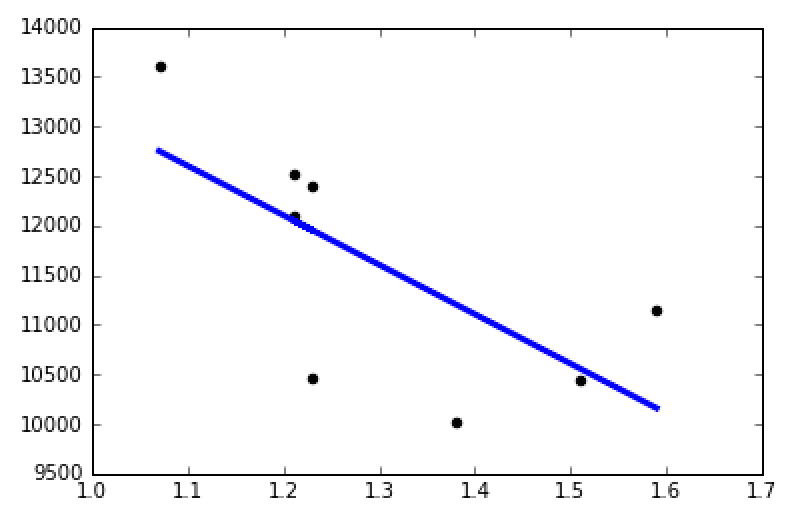
\includegraphics[width=0.4\textwidth]{lr_foreign_travels.png}}
     \qquad
    \subfloat[Domestic travels]{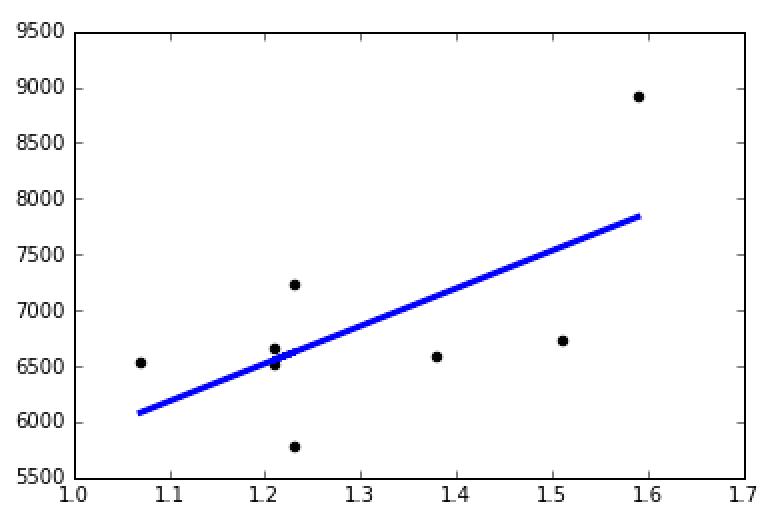
\includegraphics[width=0.4\textwidth]{lr_swiss_travels.png}}
\caption{\textit{Linear regression of foreign travels (left) and domestic travels (right) in relation to the Franc-Euro exchange rate}}
\end{figure}

We have plotted the travels abroad against the exchange rate and the graph on the left clearly shows a negative relationship. A negative relationship means, that the bigger the exchange rate, the more people travel abroad. A rising exchange rate means, that the Swiss Franc is less valuable abroad, as an exchange rate of 1.59 means, that a Euro will cost the traveller 1.59 in comparison to a lower exchange rate. We have assumed this relationship, since it is intuitive. 
\ \\

On the right side we plotted the domestic travels against the Swiss Franc. As assumed, we can see a positive relationship between domestic travels and the exchange rate. Interestingly the positive relationship is driven by the year 2008, when the exchange rate was at its highest. Before that, the dots do not clearly show a positive relationship. We can hence assume, that for domestic travels a weak Swiss Franc is less important and does not influence domestic travels to a similar extend! This finding is quite interesting, as it shows, that exchange fluctuations in the years between 2009 and 2015 did not or not strongly influence domestic travels, but had a strong impact on number of travels abroad. This is, because traveling abroad becomes considerably cheaper when deciding upon taking a trip, but does that also mean that people \textit{spend} more on travels abroad when the Swiss Franc is stronger? Interestingly and surprisingly for our group this is not the case:

%analyse more
\begin{figure}[htbp]
\centering
    \subfloat[Foreign travels]{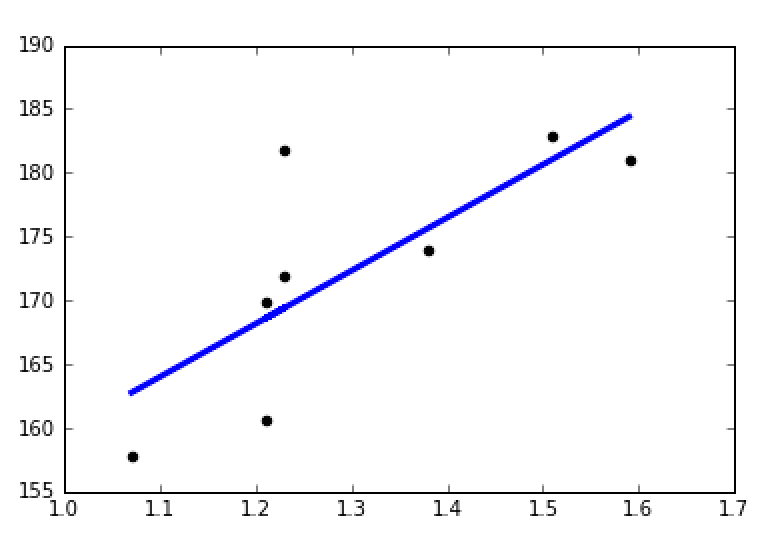
\includegraphics[width=0.4\textwidth]{lr_expenses_abroad.png}}
     \qquad
    \subfloat[Domestic travels]{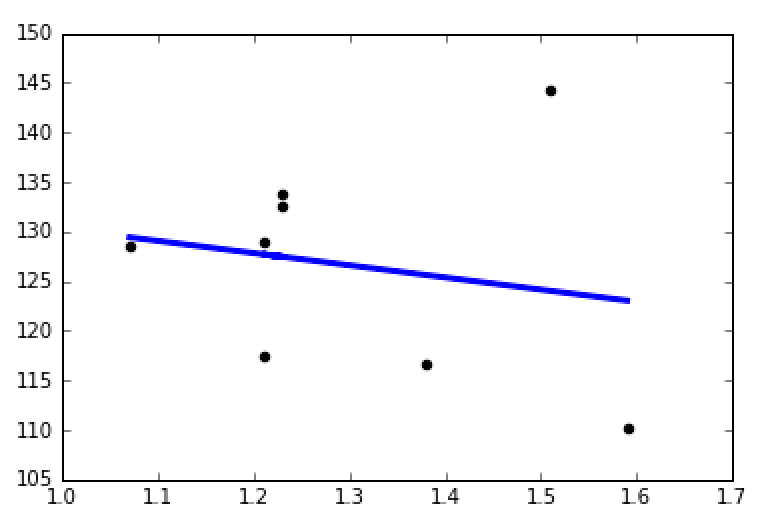
\includegraphics[width=0.4\textwidth]{lr_expenses_domestic.png}}
\caption{\textit{Linear regression of expenses abroad (left) and domestic expenses (right) in relation to the Franc-Euro exchange rate}}
\end{figure}


The stronger the Swiss Franc is, the less people spend abroad and the more they spend in Switzerland. This disapproves our assumption, that people spend more on traveling abroad (accommodation, food, transportation expenses) whenever the foreign valuta becomes cheaper. Instead the other relation is the case! A strong franc, that buys more Euros, is rather spend in Switzerland than abroad. Especially the relation between a rising exchange rate and spendings abroad is strongly positive, meaning that a Swiss Franc buying less goods abroad (higher exchange rate) is statistically rather spend abroad. What reason is there for it to be?\\ There could be a mathematical reason to it, which means that a Euro spend abroad results in a greater expense in amounts of Swiss Francs. A Swiss Franc buying more valuta mathematically results in low expenses. A Swiss Franc buying less valuta needs a greater amount in order to buy the same amounts of foreign goods. Hence the spendings rise with a rising exchange rate. This could be an explanation for the positive relationship between the relative value of the currency and the spendings abroad.
\ \\
 
 If not for mathematical reasons there also could be cultural reasons motivating to save a strong Franc rather than spending it on travels abroad. Interestingly the right graph plotting domestic expenses and exchange rate shows, that a relatively weak franc leads to less domestic travel expenses, whereas a valuable franc leads to more domestic travel expenses, which means that money is not saved but spend within the own borders. This lets us assume, that there are cultural factors influencing the decision.
%Analyze something
%\subsection{something}
\newpage
\section{Conclusion}
It is interesting to notice, that a strong franc makes people travel abroad more measured in number of travels but not spend more. We assume a mathematical issue here, which creates a bias we were not able to eliminate. A weaker Swiss Franc means, that for the same amount of goods you now need to pay a nominally higher price of Swiss Francs. The expenses hence rise with a rising exchange rate. On the other hand a weak franc does not influence number of domestic travels as much as we expected. The exchange rate hence does not have a strong effect on the number of domestic travels. 
\ \\ 

In the year 2008 we have values that could be suggested to be tested for outliers. The year 2008 brought about the financial crisis, the exchange rate hence might have been special. Taking this value out only leads to an enforcement of the results. As a conclusion we can point out that people travel abroad more the stronger the Franc, but do not or very little replace travels abroad for domestic travels, since domestic travels seem mostly exchange-rate independent. \\ Surprisingly a weak Franc does not make people spend more domestically, rather it makes them spend less on domestic travels.
\ \\
 
 In conclusion, we were right with our assumption that a strong Swiss Franc makes people travel abroad more often. The other three assumptions were disapproved: A weaker Swiss Franc does not lead to replacement of foreign travels with domestic travels, but rather is domestic travel independent of the exchange rate. The other two assumptions on the value of the Swiss Franc and its relationship to foreign and domestic spendings turned out to be exactly the opposite of what we assumed. This could be either due to a mathematical bias we could not eliminate or cultural factors. Both would need further research and exceed the scope of the given paper.

%Here comes something 

\section{Further Research}
Our research question was created in order to make scientific use of programming knowledge in Python and LaTex with the help of Github. It would hence be out of scope to eliminate the mathematical bias described above or do research on the different results. Future research should not only include the 8-year span we chose but look at a bigger time frame. Also we leave it to future research to find clear and reasonable explanations for the results we received, especially those results, that disapproved the assumptions. Finally, we would like to outline, that the given work has not only provided us with further interesting questions but also put our newly acquired programming knowledge to scientific use in form of a short paper. \\

The full automation objective was not completely attained due to the lack of coding knowledge mainly. Although our team truly believes and suggests that including the graphs as code and not images and the values of coefficients directly imported from the python modules would lead us to accomplish the goal. Conditional functions based on the coefficient's values to write specific sentences considering the scenarios could be necessary, however would not be sufficient for every case.\\
\newpage
\section{Team and Work Progress Summary}
The team consisted of three members. The team members had already some experience with basic LaTex, but little or no experience with Python and also never worked with GitHub before. After some start difficulties and a lot of trial and error, the team started to get along with the tools. Especially video tutorials online helped to navigate and operate on GitHub. 
\ \\ 

To program a working linear regression needed more time and more research. The large amount of help material available online for many problems that occurred and suggestions to embellish the code were implemented, where the solutions worked. The code was written partially in Switzerland, where two team members had the opportunity to meet physically and amended and improved remotely by the third member. Once the code was set and we got some routine in working with LaTex, we examined the result of the data regression and wrote a conclusion. 
 \ \\

Working with Python on a regular basis is necessary. Only with some routine the programming language becomes beneficial and easy to use. Our team had a steep learning curve when writing the paper and understood, that a large part of the work is invisible, namely finding bugs when pieces of code are no longer running or lead to intuitively wrong results, trying out solutions and failing forward and doing research on better and more universal ways of coding. Nevertheless our team considered this experience very valuable for our technology-led future working place and we will further enhance the knowledge we have gotten throughout the working progress with this paper.

%
%----------------------------------------------------------------------------------------------------------

% ----------------------------------------------------------------------------------------------------------


%\section{blabla} ----------------------------------------------------------------------------------------------------------

% ----------------------------------------------------------------------------------------------------------
% Literatur
% ----------------------------------------------------------------------------------------------------------



%\bibliographystyle{eehd_url}


% Literaturliste endgültig anzeigen
%\bibliography{literatur}

%-------------------


% ----------------------------------------------------------------------------------------------------------
% Anhang
% ----------------------------------------------------------------------------------------------------------

% ----------------------------------------------------------------------------------------------------------
% Literatur
% ----------------------------------------------------------------------------------------------------------


\newpage



% Literaturliste endgültig anzeigen
% Literaturliste soll im Inhaltsverzeichnis auftauchen
\section{Bibliography}
\bibliography{literatur}
% Literaturliste soll im Inhaltsverzeichnis auftauchen
Statista. (2016). "Euro (EUR) to Swiss franc (CHF) average annual exchange rate from 1999 to 2016". Retrieved on 13.12.2016 from: \\https://www.statista.com/statistics/412822/euro-to-swiss-franc-annual-average-exchange-rate/
\ \\

Swiss Federal Statistical Office. 2016. "Zeitliche Entwicklung der Reisen mit Übernachtungen, Wohnbevölkerung ab 15 Jahren". Retrieved on 15.12.2016 from: \\https://www.bfs.admin.ch/bfs/de/home/statistiken/tourismus.assetdetail.1585234.html
\ \\

Swiss National Bank. (2011). "Swiss National Bank sets minimum exchange rate at CHF 1.20 per euro". Press release.
\ \\

Swiss National Bank (2015). "Swiss National Bank discontinues minimum exchange rate and lowers interest rate to –0.75\%". Press release. 
\newpage

\bibliographystyle{eehd_url}
\bibliography{literatur}
\section{Appendix}



\subsection{Declaration of Authorship}

"We hereby certify,

\begin{itemize}
         \item  that we have written this writing sample (thesis, seminar paper, term paper or
other) without any help from others and without the use of documents and aids
other than those stated in the references, 
	  \item  that we have mentioned all the sources used and that we have cited them correctly
according to established academic citation rules, 
	  \item that the topic or parts of it are not already the object of any work or examination
of another course unless this explicitly stated, 
	  \item that we are aware that my work can be electronically checked for plagiarism and
that we hereby grant the University of St.Gallen copyright as far as this is required
for this administrative action.” 
\end{itemize}

17. Januar 2016 

Alina Asisof, Joao Matias and Carla Walker 


\end{document}




